\documentclass{article}

% set font encoding for PDFLaTeX, XeLaTeX, or LuaTeX
\usepackage{ifxetex}
\ifxetex
  \usepackage{fontspec}
\else
  \usepackage[T1]{fontenc}
  \usepackage[utf8]{inputenc}
  \usepackage{lmodern}
  \usepackage{graphicx}
  \usepackage{siunitx}
  \usepackage{amsmath}
  \graphicspath{ {images/} }
\fi

% used in maketitle
\usepackage[left=3cm,right=3cm,top=3cm,bottom=3cm]{geometry}
\title{Actividad 6}
\author{Luis Aarón Cerón Ramírez}

% Enable SageTeX to run SageMath code right inside this LaTeX file.
% documentation: http://mirrors.ctan.org/macros/latex/contrib/sagetex/sagetexpackage.pdf
% \usepackage{sagetex}

\begin{document}
\maketitle
\section{Introducción}
El siguiente trabajo tiene la finalidad de por medio del uso de herramientas computacionales resolver modelos matemáticos de situaciones físicas de manera numérica. El objetivo de este trabajo es resolver y grafícar el modelo de dos resortes con dos masas acopladas a cada resorte.

\section{Marco teórico}
El modelo consiste en dos resortes y dos pesos. Un resorte con constante $k_1$ , es sujetado al techo y colgado de este una masa $m_1$, a está masa se le colocá otro resorte con constante $k_2$, a este se le coloca otra masa $m_2$.

\begin{figure}
\centering
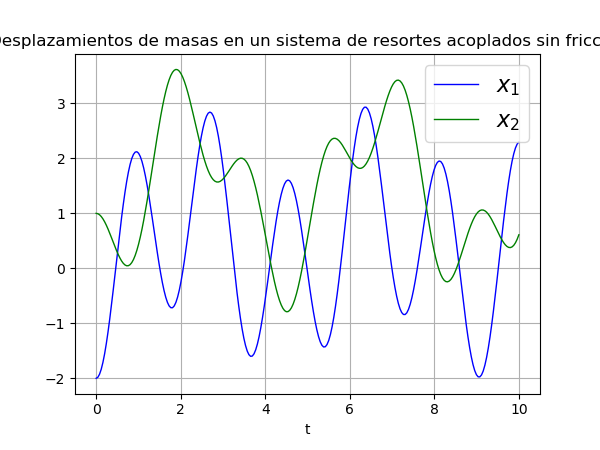
\includegraphics[scale=0.3]{two_springs.png}
\caption{Diagrama de los dos resortes acoplados}
\label{figure: Resortes acoplados }
\end{figure}

Permitiendo que el sistema se encuentre en equilibrio, medimos el desplazamiento del centro del masa de cada peso en equilibrio como función de tiempo y lo denotamos por $x_1(t)$ y $x_2(t)$.

\subsection{Asumiendo la Ley de Hooke}
Bajo la suposición de pequeñas oscilaciones, las fuerzas de restauración son de la forma:
\newline
$-k_1l_1$ y $-k_2l_2$
\newline
donde $l1$ y $l_2$ son las elongaciones de los resortes.
\newline
Observando los movimientos del sistema, tenemos entonces las siguientes ecuaciones las cuales modelan a los resortes con masas. Las ecuaciones son:

\begin{equation}
\begin{aligned}
\\m_1\ddot x_1= -k_1x_1-k_2(x_1-x_2)\\
\\m_2\ddot x_2= -k_2(x_2-x_1)\\
\end{aligned}
\end{equation}

Las cuales son dos ecuaciones diferenciales lineales de segundo orden. Para encontrar $x_1$ sin tener $x_2$, resolvemos la primer ecuación para $x_2$ obtenemos:

\begin{equation}
\begin{aligned}
\quad x_2=\frac{m_1\ddot x_1}{k_2}+\frac{(k_1+k_2)x_1}{k_2}
\end{aligned}
\end{equation}

Sustituyendo $x_2$ en la ecuación diferencial y simplificando tenemos:
\begin{equation}
\begin{aligned}
m_1m_2x_{1}^{(4)}+(m_2k_1+k_2(m_1+m_2))\ddot x_1+k_1k_2x_1=0
\end{aligned}
\end{equation}

Como se puede observar el movimiento del primer puesto es determinado por la ecuación diferencial de cuarto orden. Ahora para encontrar la ecuación que solo tenga $x_2$ resolvemos para $x_1$:
\newline
Despejando $x_1$, tenemos:
\begin{equation}
\begin{aligned}
x_1=\frac{m_2}{k_2}\ddot x_2+ x_2
\end{aligned}
\end{equation}


Sustituyendo, obtenemos una ecuación de la siguiente forma:
\begin{equation}
\begin{aligned}
m_1m_2x_{2}^{(4)}+(m_2k_1+k_2(m_1+m_2))\ddot x_2+k_1k_2x_2=0
\end{aligned}
\end{equation}

Como se puede ver es similar a la ecuación para el primer peso. El movimiento de los pesos obedecen a estas ecuaciones, y son solo la velocidad y desplazamientos iniciales las que se necesitan para determinar los casos específicos.
\newline
Tipícamente en este tipo de modelos se tienen las condiciones iniciales de $x_1(0)$ y $x_2(0)$ y las velocidades iniciales $\dot x_1(0)$ y $\dot x_2(0)$. Para resolver las ecuaciones (3) y (5),debemos conocer los valores de las derivadas $\ddot x_1(0)$, $\dddot x_1(0)$, $\ddot x_2(0)$ y $\dddot x_2(0)$. El valor de las segundas derivada estáns determinadas al evaluar las ecuaciones (2) y (4) en un tiempo t=0, mientras que los valores de las terceras derivadas se encuentran al evaluar las ecuaciones (2) y (4) en un tiempo t= 0.
\newline
Los movimientos para cualquier conjuntos de condiciones iniciales son determinados al resolver las dos ecuaciones diferenciales de cuarto orden.
\newline
Una forma alternativa de resolverlo es convirtiendo las ecuaciones de segundo orden en un sistema de cuatro ecuaciones de primer orden con los siguientes cambios $\dot x_1=u$ y $\dot x_2=v$, con lo que tenemos:
\begin{equation}
\begin{aligned}
&\dot x_1=u\\
&\dot u=-\frac{k_1}{m_1}x_1-\frac{k_2}{m_1}(x_1-x_2)\\
&\dot x_2=v\\
&\dot v= -\frac{k_2}{m_2}(x_2-x_1)\\
\end{aligned}
\end{equation}

y solo necesitamos considerar las cuatro condiciones iniciales $x_1(0)$,u(0), $x_2(0)$ y v(0).

\subsection{Algunos ejemplos con pesos idénticos}
Ahora consideremos un modelo con dos masas iguales que puede ser normalizadas como $m_1=m_2=1$. En el caso de no amortiguamiento y sin fuerzas externas, la ecuación caracteristíca de las ecuaciones diferenciales (3) y (5) es:

\begin{equation}
\begin{aligned}
m^4+(k_1+2k_2)m^2+k_1k_2=0
\end{aligned}
\end{equation}

La cual tiene raíces en:
\begin{equation}
\begin{aligned}
\pm\sqrt{-\frac{1}{2}k_1-k_2\pm\sqrt{k_1^2+4k_2^2}}
\end{aligned}
\end{equation}

\subsection{Amortiguamiento}
El tipo mas común de amortiguamiento encontrado en los principios de los cursos es el amortiguamiento viscoso, la fuerza de amortiguamiento es proporcional a la velocidad.
\newline
El amortiguamiento del primer peso depende solo de su velocidad y no de la velocidad del segundo peso y viceversa. Adicionando el termino -$\delta_1\dot x_1$ a la primer ecuación y -$\delta_2\dot x_2$ a la segunda ecuación (1). Asumimos que el coeficiente de amortiguamiemto $\delta_1$ y $\delta_2$ son pequeño. El modelo se convierte en:

\begin{equation}
\begin{aligned}
\\m_1\ddot x_1= -\delta_1\dot x_1-k_1x_1-k_2(x_1-x_2)\\
\\m_2\ddot x_2= -\delta\dot x_2-k_2(x_2-x_1)\\
\end{aligned}
\end{equation}

Para obtener una ecuación de movimiento de $x_1$ que no involucre a $x_2$, resolvemos la primer ecuación en (9) para $x_2$ y sustituir en la segunda ecuación, obteniendo:
\begin{equation}
\begin{aligned}
\\m_1m_2x_1^{4}+(m_1\delta _1+ m_2\delta _2)\dddot x_1+(m_2k_1+k_2(m_1+m_2)+\delta_1\delta_2)\ddot x_1+(k_1\delta_2+k_2(\delta_1+\delta_2)\dot x_1)+k_1k_2x_1=0
\end{aligned}
\end{equation}

y de manera similar, podemos resolver la segunda ecuación en (9) para $x_1$ y sustituir en la primer ecuación para obtener una ecuación de cuarto orden que involucra solo $x_2$, obteniendo:
\begin{equation}
\begin{aligned}
\\m_1m_2x_2^{4}+(m_1\delta _1+ m_2\delta _2)\dddot x_2+(m_2k_1+k_2(m_1+m_2)+\delta_1\delta_2)\ddot x_2+(k_1\delta_2+k_2(\delta_1+\delta_2)\dot x_2)+k_1k_2x_2=0\\
\end{aligned}
\end{equation}
Así obtenemos las mismas ecuaciones diferenciales lineales que representan a los pesos.
\section{Resultados}
Para este reporte se busco resolver los ejemplos 2.1, 2.2, 2.3 y 2.4 de manera numérica del texto con la ayuda de jupyter lab, así como obtener sus grafícas, además de obtener el error relativo como función del tiempo.

\begin{figure}[h]
\centering
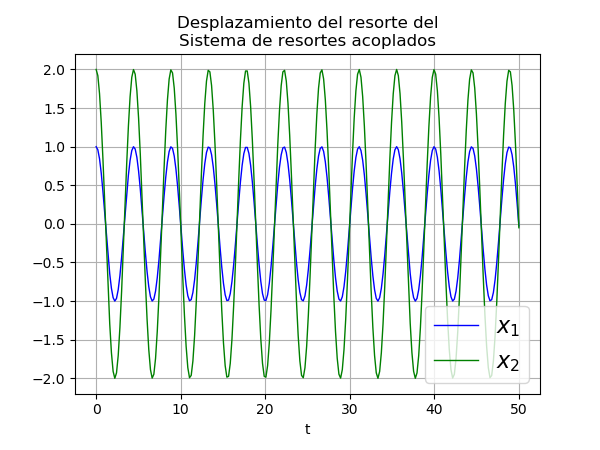
\includegraphics[scale=0.4]{r1.png}
\label{figure: Resortes acoplados }
\end{figure}


\begin{figure}[h]
\centering
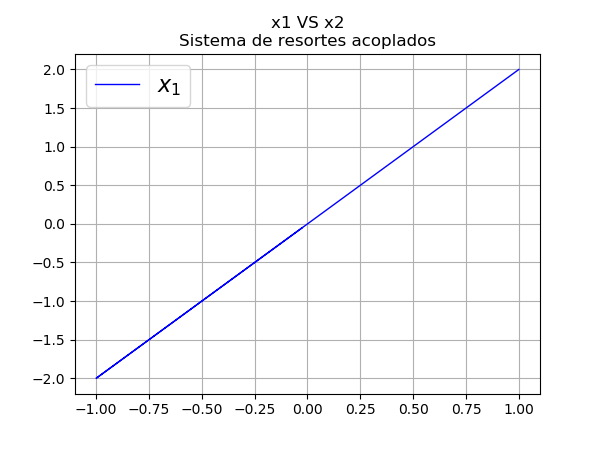
\includegraphics[scale=0.4]{r2.png}
\label{figure: Resortes acoplados }
\end{figure}

\begin{figure}
\centering
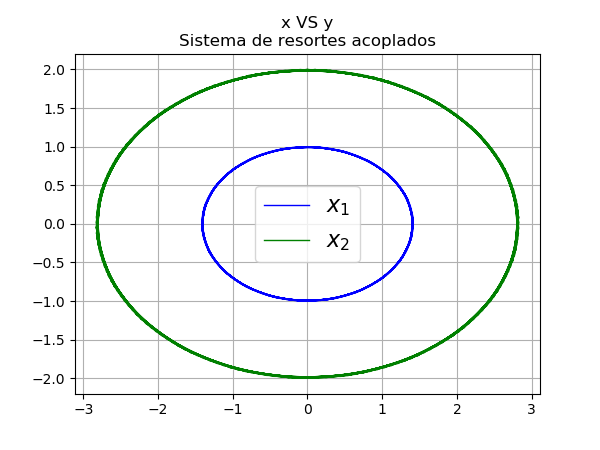
\includegraphics[scale=0.4]{r3.png}
\label{figure: Resortes acoplados }
\end{figure}

\begin{figure}[h]
\centering
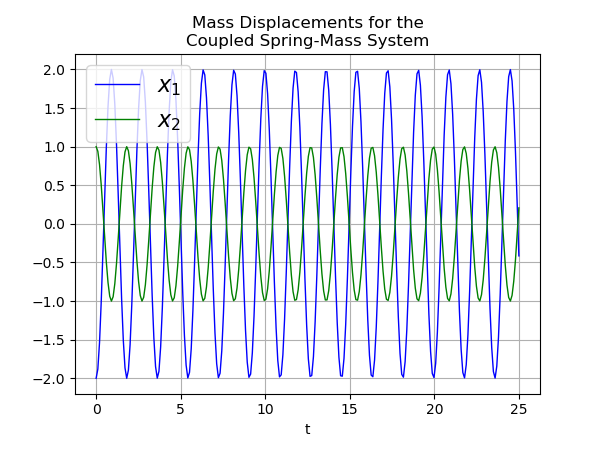
\includegraphics[scale=0.4]{r4.png}
\label{figure: Resortes acoplados }
\end{figure}

\begin{figure}[h]
\centering
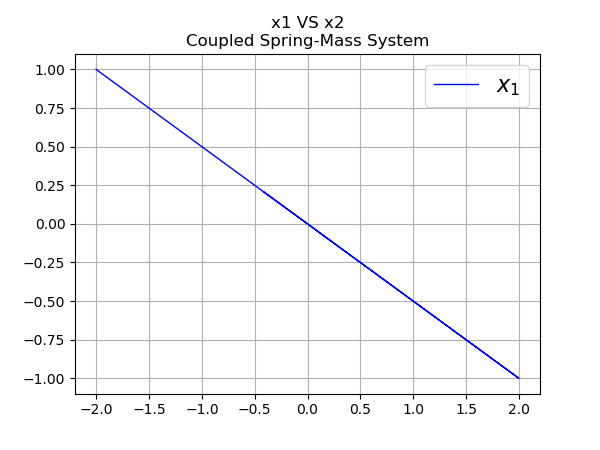
\includegraphics[scale=0.4]{r5.png}
\label{figure: Resortes acoplados }
\end{figure}

\begin{figure}[h]
\centering
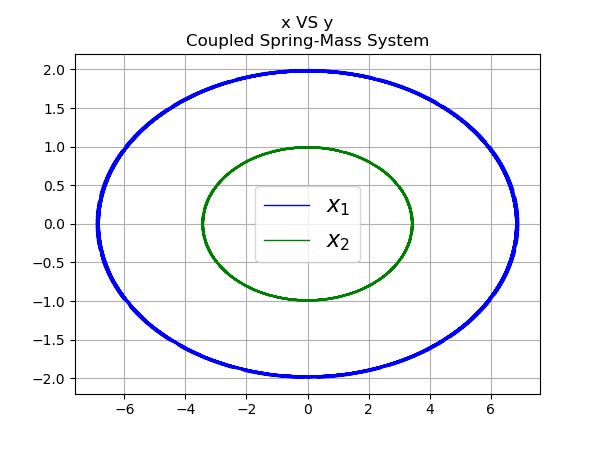
\includegraphics[scale=0.4]{r6.png}
\label{figure: Resortes acoplados }
\end{figure}

\begin{figure}[h]
\centering
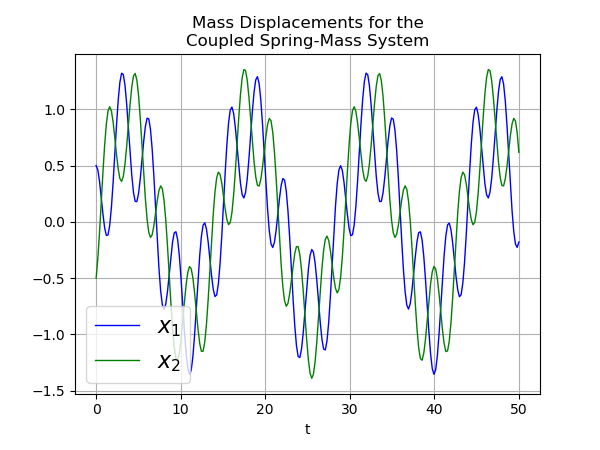
\includegraphics[scale=0.5]{r8.png}
\label{figure: Resortes acoplados }
\end{figure}

\begin{figure}[h]
\centering
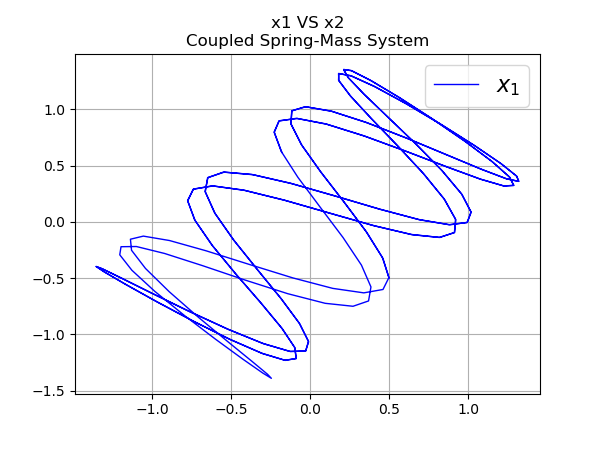
\includegraphics[scale=0.5]{r9.png}
\label{figure: Resortes acoplados }
\end{figure}

\begin{figure}[h]
\centering
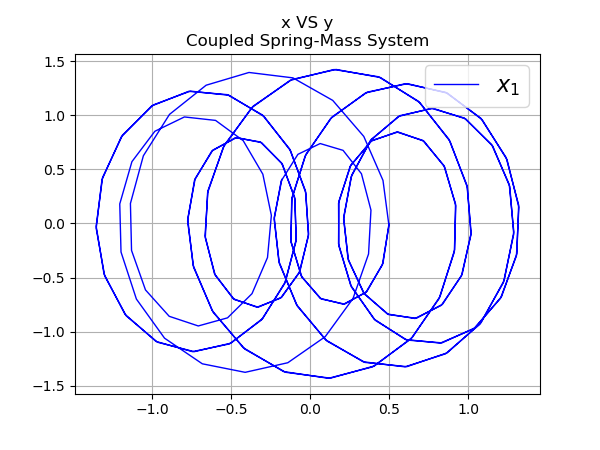
\includegraphics[scale=0.5]{r10.png}
\label{figure: Resortes acoplados }
\end{figure}

\begin{figure}[h]
\centering
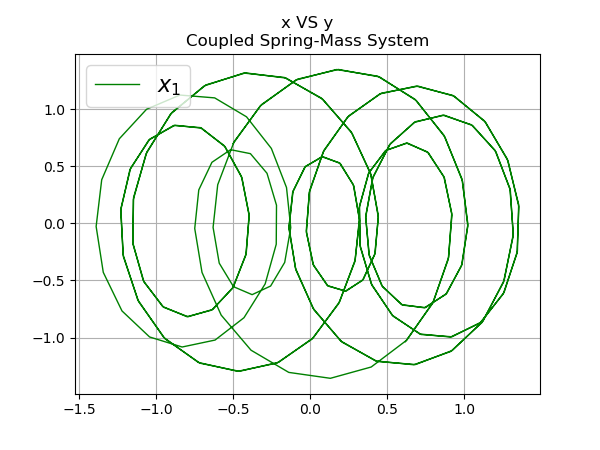
\includegraphics[scale=0.5]{r11.png}
\label{figure: Resortes acoplados }
\end{figure}

\begin{figure}[h]
\centering
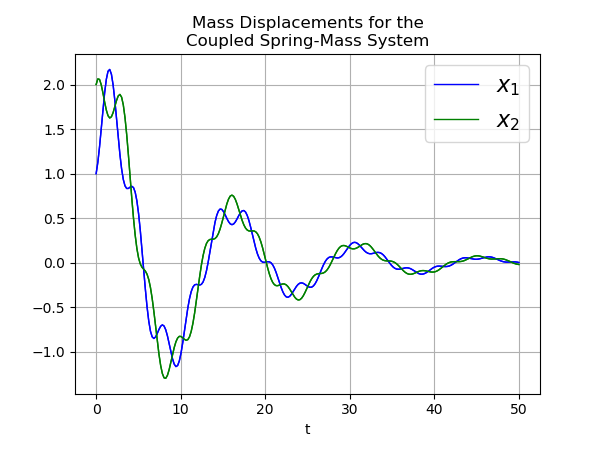
\includegraphics[scale=0.5]{r12.png}
\label{figure: Resortes acoplados }
\end{figure}

\begin{figure}[h]
\centering
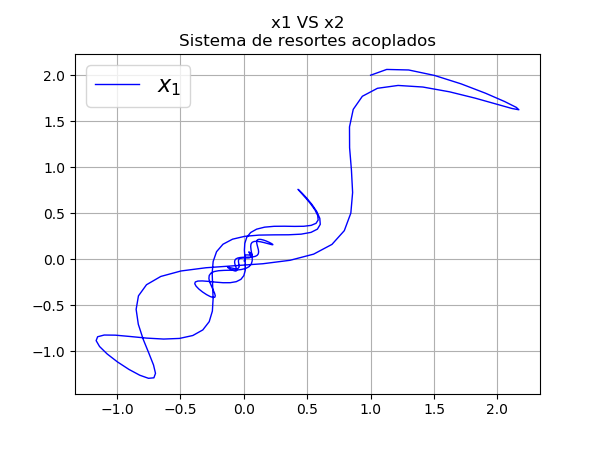
\includegraphics[scale=0.5]{r13.png}
\label{figure: Resortes acoplados }
\end{figure}

\begin{figure}[h]
\centering
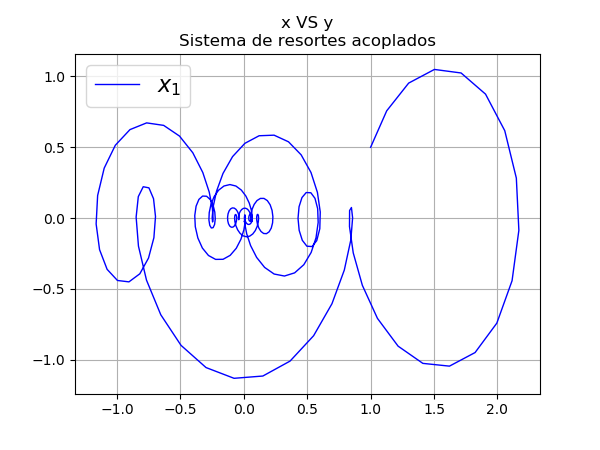
\includegraphics[scale=0.5]{r14.png}
\label{figure: Resortes acoplados }
\end{figure}

\begin{figure}[h]
\centering
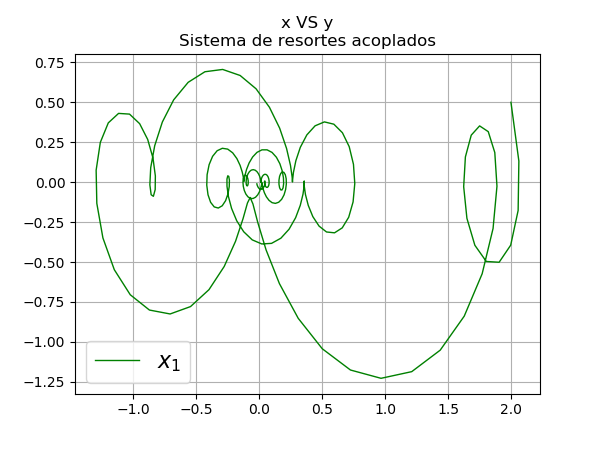
\includegraphics[scale=0.5]{r15.png}
\label{figure: Resortes acoplados }
\end{figure}





\section{Conclusión}
El uso de herramientas computacionales para resolver problemas fisícos, es una aplicación muy importantes de estas herramientas.
Este tipo de aplicaciones facilitan la resolución de problemas que de si se hicieran a mano esto seria muy cansado y complicado pues las computadoras nos brindan una gran exactitud en las operaciones. Así como las herramientas que nos brindan como la graficación, lo que nos ofrece tener muchas mas posibilidades de visualizar los comportamientos de los fenómenos.

\section{Apendice}

Preguntas antes de terminar:
\newline
¿En general te pareció interesante esta actividad de modelación matemática? ¿Qué te gustó mas? ¿Qué no te gustó?
\newline
Me parecio muy interesante el hecho de poder usar esta herramienta para facilitar el analisis, y me gusto la forma en que se puede tener una idea mejor del como se comporta el modelo por medio de las graficas.
\newline
La cantidad de material te pareció ¿bien?, ¿suficiente?, ¿demasiado?
\newline
Me parecio que tenia un poco demas, ya que eran bastantes graficas las que se tenin que hacer
\newline
¿Qué parte fue la que menos te interesó hacer?
\newline
El reporte, pues sigo teniendo problemas a la hora de colocar las imagenes
\newline
¿Cuál es tu primera impresión de Jupyter Lab?
\newline
Me parecio muy parecido a jupyter notebook en casi todo, pero debe ser porque no explore demasiado
\newline
Respecto al uso de funciones de SciPy, ¿ya habías visto integración numérica en tus cursos anteriores? ¿Cuál es tu experiencia?.
\newline
NO de esta manera, que fue una buena de complementar el trabajo
\newline
El tema de sistema de masas acopladas con resortes, ¿ya lo habías resuelto en tu curso de Mecánica 2?
\newline
no recuerdo si lo resolvi en mecanica dos pero si en mecanica teorica
\newline
¿Qué le quitarías o agregarías a esta actividad para hacerla más interesante y divertida?
\newline
menos graficas y mas modelos

\end{document}
